\chapter{Einführung in Lotus Notes/Domino}

%=================================================

\section{Was ist Lotus Notes/Domino?}
\label{sec:2allgemein}

Lotus Notes/Domino ist eine Anwendung, welche in Form einer Server/Client Architektur (Kapitel 2.3) aufgebaut ist. 
Bis zur Version 4.5 (erschienen 1996) existierte lediglich \textit{Lotus \linebreak Notes}. Mit der stärker werdenden Popularität des Internets wurde die
 Unterscheidung von Notes und Domino komplexer. 
Ab der Version 4.6 war vom \emph{Domino Designer} die Rede, zu 
diesem Zeitpunkt, war Domino jedoch nur eine Teilanwendung, welche ein Hypertext \linebreak Transfer Protocol (HTTP)-Übersetzer war. 
Diese Teilanwendung sorgte dafür, dass Inhalte von Notes-Datenbanken in Hypertext Markup Language (HTML) übersetzt wurden. 
Es wurde von nun an nicht nur in Richtung des \textit{Rich Client} (Notes Client), sondern parallel dazu auch in \linebreak Richtung des \textit{Internets}
entwickelt. 
Das gesamte Server-Bundle und nicht nur eine einzelne Teil-\linebreak anwendung, wurde ab sofort in Domino umbenannt.
Weiters wurde entschieden, dass die Seite des Clients weiterhin als Notes bezeichnet wird.
Zusammenfassend kann gesagt werden, dass Lotus Notes die Client- und Domino die Serverseite darstellt\cite{knaepper}. 

\vspace{1cm}

%=================================================


\section{Domino Designer-Kurzüberblick}
\label{sec:2allgemein}

Die Entwicklungsumgebung um Anwendungen zu entwerfen nennt sich \textit{Domino Designer}. 
In diesem wird eine Vielzahl von Design-Elementen zur Verfügung gestellt, auf welche in Kapitel 3.1 eingegangen  wird\cite{mann}.\\
Der Domino Designer stellt eine integrierte Entwicklungsumgebung zum Entwurf von Domino-Anwendungen bereit. In diesem Zusammenhang bedeutet
integriert, dass der gesamte Prozess der Anwendungsentwicklung in einem einheitlichen Rahmen und einer einheitlichen graphischen Benutzeroberfläche
durchgeführt wird.
Beginnend beim Entwurf, über die Implementierung, bis hin zur Dokumentation\cite{knaepper}.\newline
Im Domino Designer, werden die Programmiersprachen Java, JavaScript, LotusScript sowie auch die Formelsprache von Lotus Notes unterstützt.
Diese unterstützten Programmier-\linebreak sprachen, werden in Kapitel 3.3 angeführt. Damit öffnet sich das Integrated Design \linebreak
 Environment (IDE) von Domino Designer allen 
unterstützten Programmiersprachen. Somit wird ein fehlerfreies und rasches Codieren ermöglicht. Nicht zuletzt deshalb, weil ein 
syntaxsensitiver\footnote{Gibt unterschiedliche Codeelemente in einer farblichen Unterscheidung  wieder.} Editor mit Highlight-Funktionen zur
Verfügung gestellt wird\cite{mann}.\\


%=================================================
\section{Server/Client-Prinzip}
\label{sec:2allgemein}

In diesem Abschnitt wird das Server/Client Prinzip erklärt. Für detailliertere Informationen wird auf entsprechende Fachliteratur verwiesen.\newline
Anstatt die gesamte Funktionalität einer Anwendung zuzuteilen, wird eine Trennung in \linebreak \textit{mindestens} zwei logische Schichten vorgenommen.
Es ergeben sich der \textit{Server} und der \linebreak \textit{Client}. Der Server hat die Aufgabe auf Anfragen von einem oder mehreren Clients eine \linebreak
bestimmte Funktion bereitzustellen.
Das bedeutet, dass der Client Daten darstellt, welche vom Server bereitgestellt werden. Der Server kann Daten extrahieren ohne sich um die 
Darstellung \linebreak dieser zu kümmern. Diese Architektur hat den Vorteil das Ressourcen besser genutzt werden \linebreak können\cite{knaepper}.

%=================================================

\subsection{Notes Client}
\label{sec:2allgemein}


Ein Domino-System ist für die Arbeit mit mehreren verschiedenen Typen von Clients ausgerichtet. Es k\"onnen zum Beispiel Teile der Domino Funktionalit\"at 
auch von Post Office \linebreak Protocol Version 3 (POP3) - oder Internet Message Access Protocol Version 4 (IMAP) -\linebreak  f\"ahigen E-Mail-Clients  
genutzt  werden. 
Das POP3 ist ein Übertragungsprotokoll, über welches ein Client auf
E-Mails von einem Mailserver zugreifen kann\cite{pop}. Das IMAP4 ist ein Protokoll, das den Online-Zugriff auf ein 
E-Mail-Postfach ermöglicht\cite{imap}.\newline 
Es gibt nur einen Client welcher in der Lage ist alle Funktionalit\"aten von Domino zu \"ubernehmen: der \textit{Notes Client}.
Der Notes-Client ist ein grafischer Personal Information Manager (PIM).
Eine Besonderheit des Notes-Clients ist, dass er seine eigene Anwendungsentwicklung, namens \textit{Domino Designer} 
(Kapitel 3.1), bereitstellt\cite{knaepper}.


%=================================================
\subsection{Domino-Server}
\label{sec:2allgemein}

Der Kern des Domino-Servers besteht aus einem Datenbank-Server. Vergleichbar mit einem relationalen Datenbank-Server, ermöglicht dieser 
einen gleichzeitigen Zugriff für mehrere Benutzer. Es muss jedoch klar festgelegt werden, dass Notes \textit{keine} relationale Datenbank ist. 
%Vergleichbar mit relationalen Datenbank-Server, ermöglicht der Domino-Server eine Nutzung von einer Datenbank für mehrere Benutzer.
Dieser Datenbank-Server wird als \textit{Task}, welcher auf einem Domino-System läuft, bezeichnet.
Neben dieser Aufgabe werden ein Reihe von Modulen bereitgestellt, welche als separate Anwendungen beendet oder gestartet werden können\cite{knaepper}.
Von einer vollständigen Auflistung aller Server-Tasks wird in dieser Arbeit abgesehen.
\vspace{0.5cm} 


%\begin{graybox}
%\textbf{Begriffserklärung relationale Datenbank: }Bei einer relationalen Datenbank liegt die Datenbasis bzw. der Datenbestand in Form 
% einer 2-dimensionalen tabellenartigen Struktur vor, die über 
%Schlüssel (Primärschlüssel, Fremdschlüssel) miteinander in Relation (Verbindung) stehen\cite{relationalDB}.
%\end{graybox}

\begin{flushleft}
Die Tasks können in folgende Gebiete aufgeteilt werden:
\end{flushleft}

\begin{enumerate}
\item Erweiterung der Kernfunktionalität
\begin{enumerate}
\item Einige der Kernfunktionalitäten von Domino sind in Form von separaten Tasks am Server realisiert. Beispiele für diese Server-Tasks sind die
		 Volltextindizierung, der \linebreak Replikationsprozess, der Agent-Manager sowie der Mail-Router. \linebreak Volltextindizierung bedeutet, dass der
		  vollständige Text 
		  erfasst und in Einzelteilen registriert bzw. katalogisiert wird.
\end{enumerate}
\item Administrationsfunktionen
\begin{enumerate}
\item Da es umfangreich wäre die Administration manuell durchzuführen, sind einige Administrator-Tätigkeiten in Form von Server-Tasks
	beinahe vollständig \linebreak automatisiert. Es handelt sich hierbei um die Generierung von Statistiken, das \linebreak
	Komprimieren sowie
	 das Reparieren und die Verwaltung von Datenbanken.
\end{enumerate}
\item Internet-Tasks
\begin{enumerate}
\item Diese Tasks besitzen in erster Linie die Aufgabe, Domino-Funktionalität für Internet-Clients zur Verfügung zu stellen wie beispielsweise der HTTP-Task,
	aber auch der Mail-Zugriff über POP3 und der IMAP4-Task.
\end{enumerate}
\end{enumerate}


Der Server verfügt über keine graphische Benutzeroberfläche, sondern wird mittels Konsolen-Kommandos bedient. Mit diesen Kommandos können
 einzelne Server-Tasks manuell ge-\linebreak startet oder beendet werden\cite{knaepper}. Es besteht die Möglichkeit, mittels des Domino-Administrators \linebreak
(Kapitel 2.3.3) die Konfiguration über eine graphische Oberfläche vorzunehmen.


\vspace{0.1cm}

%================================================

\subsection{Domino-Administrator}
\label{sec:2allgemein}

Der Domino-Administrator ist der Administrator-Client für Notes und Domino. Er bietet \textit{Tasks} an, welche für Administrationsaufgaben
verwendet werden. Ein solcher Task ist zum Beispiel Domino Domain Monitoring (DDM).
%Hierbei wird das Konzept von DDM verfolgt.
 Mit DDM werden Überwachungsfunktionen von Domino-Servern 
durchgeführt. Ziel ist es, den Status von mehreren Domino Domänen zentral zu überblicken.\newline  
Dieser Administrator bietet Serverinformationen und Administrationsmöglichkeiten der Infrastruktur an einer zentralen Stelle. 
Für zusätzliche Informationen wird auf \cite{ebel} verwiesen.
\vspace{1cm}
%\begin{graybox}
%\textbf{\textit{Definition Administration:}} Die Administration ist die Verwaltung von Kommunikations- oder Computersystemen. Als zentrale, dezentrale oder
%verteilte Einrichtung verschafft die Administration einen Überblick über alle angeschlossenen Benutzer, über die zur Verfügung stehenden Ressourcen und 
%Programme und über die aktuellen und vergangenen Aktivitäten\cite{admin}.
%\end{graybox}
%===========================================================================================

\section{Domino-Datenbank}

Die Informationen für dieses Kapitel wurden sofern nicht anders angegeben, aus\cite{ebel} und \cite{knaepper} entnommen.
%-------------------------------

\subsection{Allgemeine Beschreibung}
\label{sec:3dominoDB}

Eine Domino Datenbank, auch als Notes Datenbank bezeichnet, enthält alle Daten und \linebreak Informationen einer Anwendung. 
Die Datenstruktur, die Funktionalität und die Oberfläche \linebreak werden durch das Design einer Anwendung festgelegt. Eine Datenbankdatei
kann als eine Art Container gesehen werden. In diesem Container sind Gestaltungs-/Design-Elemente, wie auch die Daten der Anwendung abgelegt.
Domino-Datenbanken sind die Grundbausteine einer Domino-Anwendung. Diese unterscheiden sich von klassischen Datenbanken.
Während \linebreak klassische Datenbanken eine reine Ansammlung von Daten sind, können Domino-Datenbanken auch beliebig gestaltet werden. 
Eine Domino-Datenbank ist eine Ansammlung von miteinander in sachlicher Beziehung stehenden Dokumenten. Jedes Dokument wiederum besteht  
aus einem oder mehreren Feldern\cite{knaepper}. \newline
%
%Domino-Dokumente sind mit einer relationalen Datenbank vergleichbar, mit dem Unterschied, dass bei Domino die Programmierlogik, und die
%Gestaltungselemente in Form von Dokumenten verwaltet werden.\newline
Eine Domino-Datenbank ist \textit{keine} Datenbank im herk\"ommlichen Sinn, sondern eine fertige \linebreak Applikation, welche eine spezielle
Ablaufumgebung ben\"otigt. Diese kann entweder der Notes-Client (Kapitel 2.3.1) oder ein Domino-Server (Kapitel 2.3.2) sein\cite{knaepper}.
\vspace{0.5cm}
%\begin{graybox}
%\textbf{Information: }Mit der Einführung der Version 8, wurden Datenbanken in Anwendungen umbenannt.
%\end{graybox}
%============================

\subsubsection{Relationale Datenbank versus Domino-Datenbank}
\label{sec:3dominoDB}
Gegen\"uber klassischen relationalen Datenbanken, ist eine Domino Datenbank besonders f\"ur eine flexible Verwaltung von unstrukturierten Inhalten
geeignet.
Eine Domino-Datenbank hat gegenüber einer relationalen Datenbank einige Vorteile. Insbesondere, wenn es sich um die Verwaltung von unstrukturierten 
Inhalten handelt, besitzt die Domino-Datenbank Vorteile.\\
Es können Inhalte von beliebigen Typen wie zum Beispiel
\begin{itemize}
\item Office Dokumente,
\item Applets\footnote{Ein Applet ist ein im Web-Browser laufendes Java-Programm.},
\item Bilder,
\item oder Videos
\end{itemize}
verwaltet werden. Hierbei kann die Struktur von einzelnen Datensätzen verändert werden\cite{knaepper}. 
Zu den Vorteilen einer Domino-Datenbank gehört, dass mit Rich-Text-Feldern jede \linebreak erdenkliche Information, wie zum Beispiel
Texte, Bilder, Tabellen, Grafiken sowie Object \linebreak Linking and Embedding (OLE)-Objekte oder ganze Dateien abgelegt werden können.
OLE ist ein Objektsystem und Protokoll, das die Zusammenarbeit unterschiedlicher (OLE-fähiger) Applikationen ermöglicht\cite{ebel}. 

Der Nachteil dieser Anwendungen ist, dass es keine Sicherstellung der Datenqualität gibt. 
Ein weiterer Nachteil ist, dass keine automatische Vermeidung von Redundanzen \linebreak vorhanden ist. 
Darum soll eine Domino-Datenbank nicht eingesetzt werden, wenn es sich um die Verwaltung von großen Mengen von strukturierten Daten handelt. 
Wie in Kapitel 1.1 erwähnt, handelt es sich um eine Groupware-Anwendung. Aus diesem Grund kann ausgeschlossen \linebreak werden, dass ein 
solcher Fall eintritt\cite{knaepper}.\newline

%============================
\subsection{Datenbankarchitektur}
\label{sec:3dominoDB}

Physisch gesehen wird eine Domino-Datenbank durch eine Datei mit \textit{.nsf}-Endung abgebildet. Die Endung
\textit{.nsf} steht für Notes Storage Facility. Wie dem Namen zu entnehmen ist handelt es sich um die Möglichkeit Notizen (Notes) aufzunehmen.
 Diese Notizen, oder in anderen Worten gesagt, Dokumente oder Datensätze enthalten Felder, welche mit Daten oder Informationen gefüllt sind\cite{ebel}.

\begin{figure}[H]
  \centerline{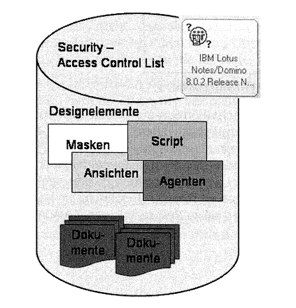
\includegraphics[scale=0.7]{pics/DB_container}}
  \caption[Elemente einer Domino-Datenbank]{\label{FiG:Elemente einer Domino-Datenbank }
  Elemente einer Domino-Datenbank\cite{ebel}}
\end{figure}
%\begin{flushleft}
Die Abbildung 2.1 zeigt den Aufbau einer Domino-Datenbank. Es ist erkennbar, dass Design-Elemente und Dokumente in einem gemeinsamen Container
abgelegt sind. 
%\end{flushleft}


\vspace{1cm}
%\begin{graybox}
%\textbf{Information zu Dokumenten: }Dokumente bestehen aus Text, Feldern, Zahlen, Grafiken etc. Der Benutzer kann Daten eingeben, von Formeln
%automatisch berechnen lassen, von anderen Anwendungen Daten importieren oder eine Verknüpfung einer anderen Anwendung erstellen. Dabei werden die
%Daten dynamisch aktualisiert\cite{ebel}.
%\end{graybox}

%============================

\subsection{Datenbank-Informationen}
\label{sec:3dominoDB}

Die Datenbank-Informationen umfassen alle Eigenschaften einer Datenbank. Diese \linebreak Eigenschaften sind für die gesamte Datenbank gültig.
\begin{flushleft}
Zu diesen Informationen gehören unter anderem:
\end{flushleft}
\begin{itemize}
\item Identifikation einer  Datenbank,
\item Datenbanktitel,
\item Name der Datenbankdatei,
\item maximale Größe,
\item verfügbarer Speicherplatz. 
\end{itemize}
Die Eigenschaftseinstellungen werden beim Erstellen einer Datenbank durch den Ersteller \linebreak spezifisch angegeben. 
Weiters besteht auch die Möglichkeit, dass die Einstellungen durch das System automatisch vorgenommen werden.

%============================
\subsubsection{Design-Elemente}
\label{sec:3dominoDB}

Wie in Kapitel 2.4.1 erwähnt, besteht eine Domino-Datenbank nicht nur aus Daten sondern bietet auch eine Reihe von Gestaltungs- oder Design-Elementen.
Informationen über Design-Elemente werden in Dokumenten verwaltet. Dies bietet die Möglichkeit sie zu kopieren, löschen oder replizieren zu
können. Die notwendigen Design-Elemente für das Template, werden in Kapitel 3.2 aufgelistet und beschrieben. 

%============================

\subsubsection{Daten}
\label{sec:3dominoDB}

Die Verwaltung der eigentlichen Daten wird, wie auch die der Design-Elemente, über \linebreak Dokumente erledigt. 
Ein Dokument ist eine autonome Einheit, welche die Struktur eigenständig verwaltet. Dies hat den Vorteil, dass die Größe und die Struktur des 
Dokumentes zu jedem Zeitpunkt beliebig verändert werden kann. Dokumente besitzen die Funktion sich wie ein Behälter für Grafiken, Texte, Objekte
oder multimediale Daten zu verhalten. Diese Funktionalität wird als \textit{compound-document} bezeichnet und ist für relationalen Datenbanken,
nur über umständliche Wege realisierbar. Ein compound-document ist ein aus mehreren Objekten zusammengesetztes Dokument\cite{wind}. 

\vspace{0.5cm}

\begin{graybox}
\textit{In einer dokumentorientierten Umgebung wie Notes bilden compound-documents die Grundlage einer jeden Internet-/Groupware-/Workflow-Anwendung\cite{knaepper}.}
\end{graybox}

%============================
\subsection{Zugriffs-Möglichkeiten auf eine Domino-Datenbank}



Um Anwendungen, welche sich auf dem Domino-Server befinden, auszuführen, gibt es unterschiedliche Möglichkeiten.
In diesem Kapitel werden diese Zugriffsarten behandelt.\newline

%Eine Anwendung welche im Domino Administrator erstellt wurde, kann auf unterschiedliche Arten aufgerufen und bearbeitet werden.


\subsubsection{Benutzer Zugriff}
\label{sec:5webzugriff}


Im Gegensatz zu Lotus Domino stellt Lotus Notes die Seite des Clients dar. Der Notes Client verwaltet die Benutzeroberfläche und ist für die 
grafische Aufbereitung der Daten zuständig.\newline
Notes Clients interagieren mit Datenbanken, welche sich am Domino-Server befinden, in unterschiedlicher Weise.
Grundsätzlich gibt es zwei mögliche Zugriffsarten:
\begin{itemize}
\item Zugriff mit Notes Client, 
\item Zugriff über einen Web-Browser, zum Beispiel mit Internet Explorer oder Mozilla Firefox. 
\end{itemize}



\subsubsection{Zugriff über Notes Client}
\label{sec:5webzugriff}

Für die Kommunikation eines Notes Clients mit einem Domino Server werden Protokolle benötigt. Diese Kommunikation wird entweder über Notes-Protokolle
(Notes Remote Procedure Call (NRPC)) oder über Internet-Protokolle wie POP3 oder IMAP4 abgewickelt (Kapitel 2.3.1). \linebreak Notes RPC ist eine 
Variante von Remote Procedure Call und kann über Protokolle wie TCP/IP (Transmission Control Protocol/Internet Protocol) geroutet werden.
Der Anwender greift dabei auf Datenbanken, auf die er die Zugriffsberechtigung besitzt, zu. 
Diese Datenbanken werden als Datenbanksymbole auf dem Arbeitsplatz im Notes Client abgelegt (Abbildung 2.2)\cite{ebel}.

\begin{figure}[H]
    \centerline{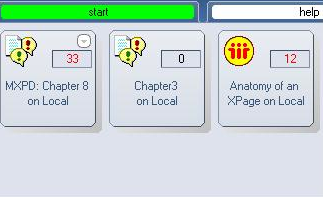
\includegraphics[scale=0.5]{pics/Client_kacheln}}
    \caption[Darstellung einer Datenbank im Notes Client]{\label{FiG:Darstellung einer Datenbank im Notes Client}
	Datenbanken im Notes Client}
\end{figure}


\subsubsection{Zugriff über Web-Browser}
\label{sec:5webzugriff}

Um den Zugriff über einen Browser zu ermöglichen, wird vorausgesetzt, dass sich die \linebreak
Anwendung auf einem Domino-Server befindet, welcher als Webserver
agiert\cite{ebel}.
Die eindeutige Adresse einer Ressource oder eines Dokuments im Internet bezeichnet man als Uniform Re-\linebreak
source Locator (URL). Eine URL setzt sich nach 
bestimmten syntaktischen Regeln zusammen. Diese Regeln enthalten unter anderem den Namen des Host-Rechners und den Pfad bzw.
den Namen des Dokuments\cite{knaepper}.\\
\newline
Eine URL kann sich zum Beispiel wie folgt zusammensetzen:
\begin{equation}
http://s124/work/template.nsf/default.xsp
\end{equation} 

In diesem Beispiel wird eine XPage, namens \textit{default}, aufgerufen. Diese XPage ist ein Teil der Datenbank \textit{template} und \textit{work} ist das
Verzeichnis auf dem Server \textit{s124}, der zu diesem Dokument führt. Hierbei handelt es sich um einen Webserver, welcher HTTP 
zum Informationsaustausch benutzt. Das hier angeführte Beispiel, beschränkt sich auf den lokalen Zugriff über das Intranet.\\
\newline
 Wird der Zugriff über das Internet durchgeführt, so setzt sich die URL wie folgt zusammen:
\begin{equation}
http://server.domain.com/work/template.nsf/default.xsp
\end{equation} 


Die sich auf dem Domino Server befindenden Datensätze können somit über einen Web-Browser aufgerufen werden. 
 




